\documentclass[12pt]{report}
\usepackage[utf8]{inputenc}
\usepackage{graphicx}
\usepackage{wrapfig}
\usepackage{ngerman} % ngerman -> neue Rechtschreibung
\usepackage{acronym}
\usepackage{fancyhdr}
\usepackage{pdfpages}
\usepackage{hyperref}
% Bei Bachelor-/Masterarbeiten darf wegen der Bindung left auf 4.5 - 6 gestellt werden
\usepackage[a4paper,left=2.5cm,right=2.5cm,top=2.5cm,bottom=2cm]{geometry}
\usepackage[onehalfspacing]{setspace}
% Zitationsstil
\bibliographystyle{apalike}
\graphicspath{ {./images/} }

% \pagestyle{fancyplain}
% \fancyfoot[EL,OR]{\thepage}

\pagestyle{fancy}
\fancyhf{}
\fancyhead[R]{\nouppercase{\leftmark}}
\fancyfoot[R]{\thepage}
\setlength{\headheight}{15pt}

\fancypagestyle{plain}{ % Damit Seiten mit plain pagestyle auch die Seitennummerierung rechts haben
  \fancyhf{} % remove everything
  \renewcommand{\headrulewidth}{0pt} % remove lines
  \fancyfoot[R]{\thepage}
}

\begin{titlepage}
    \title{
    {\centering
\includegraphics[width=0.7\textwidth]{fh_logo}\newline}\\    
    {Microservices}\\
    {\large Eine Übersichtsarbeit angefertigt im Rahmen des Moduls Schlüsselkompetenzen III}\\
    \vfill
    {
    \begin{tabular}{ c c }
        \small Vorgelegt von: & \small Felix Schulze Sindern \\ 
        \small Matrikelnummer: & \small 965396 \\  
        \small Abgabedatum: & \small 30. April 2020 \\
    \end{tabular}
   
    }
}
\date{} % Leeres Datum muss verwendet werden, sonst wird das Datum komisch angehängt
\author{} % Sonst wird eine Warnung geworfen

\end{titlepage}

\begin{document}
\pagenumbering{Roman}
\maketitle

\chapter*{Abstract}
Auch gibt es niemanden, der den Schmerz an sich liebt, sucht oder wünscht, nur, weil er Schmerz ist,
es sei denn, es kommt zu zufälligen Umständen, in denen Mühen und Schmerz ihm große Freude bereiten
können. Um ein triviales Beispiel zu nehmen, wer von uns unterzieht sich je anstrengender körperlicher
Betätigung, außer um Vorteile daraus zu ziehen? Aber wer hat irgend ein Recht, einen Menschen zu
tadeln, der die Entscheidung trifft, eine Freude zu genießen, die keine unangenehmen Folgen hat,
oder einen, der Schmerz vermeidet, welcher keine daraus resultierende Freude nach sich zieht?
Auch gibt es niemanden, der den Schmerz an sich liebt, sucht oder wünscht, nur, weil er Schmerz ist,
es sei denn, es kommt zu zufälligen Umständen, in denen Mühen und Schmerz ihm große Freude bereiten
können. Um ein triviales Beispiel zu nehmen, wer von uns unterzieht sich je anstrengender körperlicher
Betätigung, außer um Vorteile daraus zu ziehen? Aber wer hat irgend ein Recht, einen Menschen zu
tadeln, der die Entscheidung trifft, eine Freude zu genießen, die keine unangenehmen Folgen hat,
oder einen, der Schmerz vermeidet, welcher keine daraus resultierende Freude nach sich zieht? Auch
gibt es niemanden, der den Schmerz an sich liebt, sucht oder wünscht, nur, weil er Schmerz ist, es
sei denn, es kommt zu zufälligen Umständen, in denen Mühen und Schmerz ihm große Freude bereiten
können.

\tableofcontents
\listoffigures
\addcontentsline{toc}{chapter}{Abbildungsverzeichnis}
\newpage

\section*{\huge Abkürzungsverzeichnis}
\addcontentsline{toc}{chapter}{Abkürzungsverzeichnis}
\thispagestyle{plain}
\begin{acronym}
    \acro{KDE}{K Desktop Environment}
    \acro{SQL}{Structured Query Language}
    \acro{Bash}{Bourne-again shell}
    \acro{JDK}{Java Development Kit}
    \acro{VM}{Virtuelle Maschine}
    \acrodefplural{VM}[VMs]{Virtuelle Maschinen}
    \acro{I2C}[I²C]{Inter-Integrated Circuit}
\end{acronym}

\chapter{Einführung}
\pagenumbering{arabic}
Auch gibt es niemanden, der den Schmerz an sich liebt, sucht oder wünscht, nur, weil er Schmerz ist,
es sei denn, es kommt zu zufälligen Umständen, in denen Mühen und Schmerz ihm große Freude bereiten
können. Um ein triviales Beispiel zu nehmen, wer von uns unterzieht sich je anstrengender körperlicher
Betätigung, außer um Vorteile daraus zu ziehen? Aber wer hat irgend ein Recht, einen Menschen zu
tadeln, der die Entscheidung trifft, eine Freude zu genießen, die keine unangenehmen Folgen hat,
oder einen, der Schmerz vermeidet, welcher keine daraus resultierende Freude nach sich zieht?
Auch gibt es niemanden, der den Schmerz an sich liebt, sucht oder wünscht, nur, weil er Schmerz ist,
es sei denn, es kommt zu zufälligen Umständen, in denen Mühen und Schmerz ihm große Freude bereiten
können. Um ein triviales Beispiel zu nehmen, wer von uns unterzieht sich je anstrengender körperlicher
Betätigung, außer um Vorteile daraus zu ziehen? Aber wer hat irgend ein Recht, einen Menschen zu
tadeln, der die Entscheidung trifft, eine Freude zu genießen, die keine unangenehmen Folgen hat,
oder einen, der Schmerz vermeidet, welcher keine daraus resultierende Freude nach sich zieht? Auch
gibt es niemanden, der den Schmerz an sich liebt, sucht oder wünscht, nur, weil er Schmerz ist, es
sei denn, es kommt zu zufälligen Umständen, in denen Mühen und Schmerz ihm große Freude bereiten
können.

\section{Verwendung von Abkürzungen}
Beim ersten mal wird automatisch die Langform verwendet: \ac{KDE}. Bei weiteren Verwenden des Befehlt wird nur die Kurzform verwendet: \ac{KDE}. Es kann der Plural referenziert werden: \acp{KDE}.
Standardmäßig wird einfach der Buchstabe s angehängt. Wenn das nicht passend ist wie bei \ac{VM}, muss der Plural exlpizit spezifiziert werden \acp{VM}.

\section{Grundlagen}
Auch gibt es niemanden, der den Schmerz an sich liebt, sucht oder wünscht, nur, weil er Schmerz ist,
es sei denn, es kommt zu zufälligen Umständen, in denen Mühen und Schmerz ihm große Freude bereiten
können.
\subsection{Grundlagen der Grundlagen}
Um ein triviales Beispiel zu nehmen, wer von uns unterzieht sich je anstrengender körperlicher
Betätigung, außer um Vorteile daraus zu ziehen? Aber wer hat irgend ein Recht, einen Menschen zu
tadeln, der die Entscheidung trifft, eine Freude zu genießen, die keine unangenehmen Folgen hat,
oder einen, der Schmerz vermeidet, welcher keine daraus resultierende Freude nach sich zieht?
Auch gibt es niemanden, der den Schmerz an sich liebt, sucht oder wünscht, nur, weil er Schmerz ist,
es sei denn, es kommt zu zufälligen Umständen, in denen Mühen und Schmerz ihm große Freude bereiten
können.
\subsubsection{Grundlagen  der Grundlagen der Grundlagen}
Um ein triviales Beispiel zu nehmen, wer von uns unterzieht sich je anstrengender körperlicher
Betätigung, außer um Vorteile daraus zu ziehen? Aber wer hat irgend ein Recht, einen Menschen zu
tadeln, der die Entscheidung trifft, eine Freude zu genießen, die keine unangenehmen Folgen hat,
oder einen, der Schmerz vermeidet, welcher keine daraus resultierende Freude nach sich zieht? Auch
gibt es niemanden, der den Schmerz an sich liebt, sucht oder wünscht, nur, weil er Schmerz ist, es
sei denn, es kommt zu zufälligen Umständen, in denen Mühen und Schmerz ihm große Freude bereiten
können.

\chapter{Titel Kapitel zwei}
Auch gibt es niemanden, der den Schmerz an sich liebt, sucht oder wünscht, nur, weil er Schmerz ist,
es sei denn, es kommt zu zufälligen Umständen, in denen Mühen und Schmerz ihm große Freude bereiten
können. Um ein triviales Beispiel zu nehmen, wer von uns unterzieht sich je anstrengender körperlicher
Betätigung, außer um Vorteile daraus zu ziehen? Aber wer hat irgend ein Recht, einen Menschen zu
tadeln, der die Entscheidung trifft, eine Freude zu genießen, die keine unangenehmen Folgen hat,
oder einen, der Schmerz vermeidet, welcher keine daraus resultierende Freude nach sich zieht?
\section{Unterkapitel}
Auch gibt es niemanden, der den Schmerz an sich liebt, sucht oder wünscht, nur, weil er Schmerz ist,
es sei denn, es kommt zu zufälligen Umständen, in denen Mühen und Schmerz ihm große Freude bereiten
können.
\begin{figure}[h] % der Parameter h ist wichtig, sonst wird die Abbildung auf das Ende der Seite geschoben
    
\includegraphics[width=0.5\textwidth]{fh_logo}
    \caption{Beschriftung, die auch im Abbildungsverzeichnis auftaucht.}
\end{figure}
Um ein triviales Beispiel zu nehmen, wer von uns unterzieht sich je anstrengender körperlicher
Betätigung, außer um Vorteile daraus zu ziehen? Aber wer hat irgend ein Recht, einen Menschen zu
tadeln, der die Entscheidung trifft, eine Freude zu genießen, die keine unangenehmen Folgen hat,
oder einen, der Schmerz vermeidet, welcher keine daraus resultierende Freude nach sich zieht? Auch
gibt es niemanden, der den Schmerz an sich liebt, sucht oder wünscht, nur, weil er Schmerz ist, es
sei denn, es kommt zu zufälligen Umständen, in denen Mühen und Schmerz ihm große Freude bereiten
können. Aber wer hat irgend ein Recht, einen Menschen zu
tadeln, der die Entscheidung trifft, eine Freude zu genießen, die keine unangenehmen Folgen hat,
oder einen, der Schmerz vermeidet, welcher keine daraus resultierende Freude nach sich zieht? Auch
gibt es niemanden, der den Schmerz an sich liebt, sucht oder wünscht, nur, weil er Schmerz ist, es
sei denn, es kommt zu zufälligen Umständen, in denen Mühen und Schmerz ihm große Freude bereiten
können. 

\chapter{Titel Kapitel drei}
Auch gibt es niemanden, der den Schmerz an sich liebt, sucht oder wünscht, nur, weil er Schmerz ist,
es sei denn, es kommt zu zufälligen Umständen, in denen Mühen und Schmerz ihm große Freude bereiten
können. 
\begin{wrapfigure}{r}{0.7\textwidth}
    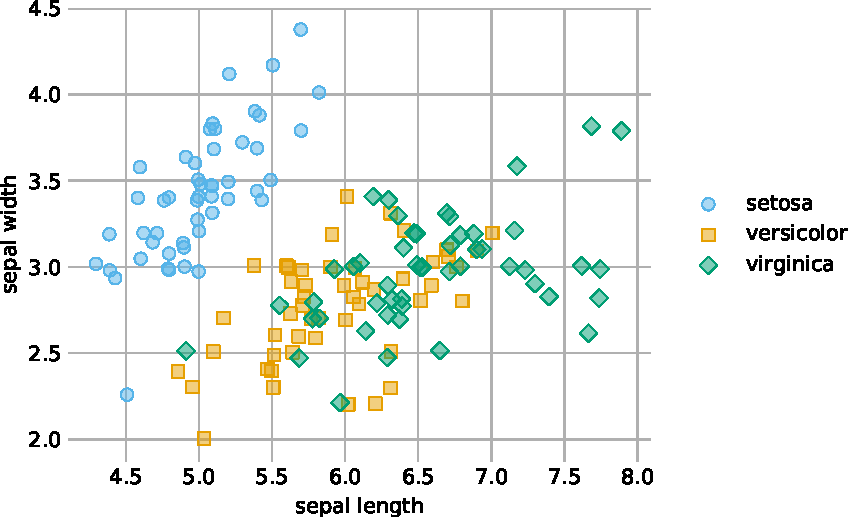
\includegraphics[width=0.7\textwidth]{iris}
    \caption{Sexy Matplotlib Diagramm}
\end{wrapfigure}
Um ein triviales Beispiel zu nehmen, wer von uns unterzieht sich je anstrengender körperlicher
Betätigung, außer um Vorteile daraus zu ziehen? Aber wer hat irgend ein Recht, einen Menschen zu
tadeln, der die Entscheidung trifft, eine Freude zu genießen, die keine unangenehmen Folgen hat,
oder einen, der Schmerz vermeidet, welcher keine daraus resultierende Freude nach sich zieht?
Auch gibt es niemanden, der den Schmerz an sich liebt, sucht oder wünscht, nur, weil er Schmerz ist,
es sei denn, es kommt zu zufälligen Umständen, in denen Mühen und Schmerz ihm große Freude bereiten
können. Um ein triviales Beispiel zu nehmen, wer von uns unterzieht sich je anstrengender körperlicher
Betätigung, außer um Vorteile daraus zu ziehen?\cite{Gamma.2015} Aber wer hat irgend ein Recht, einen Menschen zu
tadeln, der die Entscheidung trifft, eine Freude zu genießen, die keine unangenehmen Folgen hat,
oder einen, der Schmerz vermeidet, welcher keine daraus resultierende Freude nach sich zieht? Auch
gibt es niemanden, der den Schmerz an sich liebt, sucht oder wünscht, nur, weil er Schmerz ist, es
sei denn, es kommt zu zufälligen Umständen, in denen Mühen und Schmerz ihm große Freude bereiten
können.

\chapter{Titel Kapitel vier}
Auch gibt es niemanden, der den Schmerz an sich liebt, sucht oder wünscht, nur, weil er Schmerz ist,
es sei denn, es kommt zu zufälligen Umständen, in denen Mühen und Schmerz ihm große Freude bereiten
können. Um ein triviales Beispiel zu nehmen, wer von uns unterzieht sich je anstrengender körperlicher
Betätigung, außer um Vorteile daraus zu ziehen? Aber wer hat irgend ein Recht, einen Menschen zu
tadeln, der die Entscheidung trifft, eine Freude zu genießen, die keine unangenehmen Folgen hat,
oder einen, der Schmerz vermeidet, welcher keine daraus resultierende Freude nach sich zieht?
Auch gibt es niemanden, der den Schmerz an sich liebt, sucht oder wünscht, nur, weil er Schmerz ist,
es sei denn, es kommt zu zufälligen Umständen, in denen Mühen und Schmerz ihm große Freude bereiten
können. Um ein triviales Beispiel zu nehmen, wer von uns unterzieht sich je anstrengender körperlicher
Betätigung, außer um Vorteile daraus zu ziehen? Aber wer hat irgend ein Recht, einen Menschen zu
tadeln, der die Entscheidung trifft, eine Freude zu genießen, die keine unangenehmen Folgen hat,
oder einen, der Schmerz vermeidet, welcher keine daraus resultierende Freude nach sich zieht? Auch
gibt es niemanden, der den Schmerz an sich liebt, sucht oder wünscht, nur, weil er Schmerz ist, es
sei denn, es kommt zu zufälligen Umständen, in denen Mühen und Schmerz ihm große Freude bereiten
können.



\chapter{Fazit}
Auch gibt es niemanden, der den Schmerz an sich liebt, sucht oder wünscht, nur, weil er Schmerz ist,
es sei denn, es kommt zu zufälligen Umständen, in denen Mühen und Schmerz ihm große Freude bereiten
können. Um ein triviales Beispiel zu nehmen, wer von uns unterzieht sich je anstrengender körperlicher
Betätigung, außer um Vorteile daraus zu ziehen?
\begin{wrapfigure}{r}{0.5\textwidth}
    
\includegraphics[width=0.5\textwidth]{fh_logo}
    \caption{Inline Logo der FH Münster}
\end{wrapfigure}
Aber wer hat irgend ein Recht, einen Menschen zu
tadeln, der die Entscheidung trifft, eine Freude zu genießen, die keine unangenehmen Folgen hat,
oder einen, der Schmerz vermeidet, welcher keine daraus resultierende Freude nach sich zieht?
Auch gibt es niemanden, der den Schmerz an sich liebt, sucht oder wünscht, nur, weil er Schmerz ist,
es sei denn, es kommt zu zufälligen Umständen, in denen Mühen und Schmerz ihm große Freude bereiten
können.\cite[S.~150]{Wolff.2018}Um ein triviales Beispiel zu nehmen, wer von uns unterzieht sich je anstrengender körperlicher
Betätigung, außer um Vorteile daraus zu ziehen? Aber wer hat irgend ein Recht, einen Menschen zu
tadeln, der die Entscheidung trifft, eine Freude zu genießen, die keine unangenehmen Folgen hat,
oder einen, der Schmerz vermeidet, welcher keine daraus resultierende Freude nach sich zieht? Auch
gibt es niemanden, der den Schmerz an sich liebt, sucht oder wünscht, nur, weil er Schmerz ist, es
sei denn, es kommt zu zufälligen Umständen, in denen Mühen und Schmerz ihm große Freude bereiten
können.

%Literaturverzeichnis
\addcontentsline{toc}{chapter}{Literaturverzeichnis}
\bibliography{Literatur}

\appendix
\chapter{Titel des Anhangs}
Lorem ipsum dolor sit amet, consetetur sadipscing elitr, sed diam nonumy eirmod tempor invidunt ut labore et dolore magna aliquyam erat, sed diam voluptua. At vero eos et accusam et justo duo dolores et ea rebum. Stet clita kasd gubergren, no sea takimata sanctus est Lorem ipsum dolor sit amet. Lorem ipsum dolor sit amet, consetetur sadipscing elitr, sed diam nonumy eirmod tempor invidunt ut labore et dolore magna aliquyam erat, sed diam voluptua. At vero eos et accusam et justo duo dolores et ea rebum. Stet clita kasd gubergren, no sea takimata sanctus est Lorem ipsum dolor sit amet. Lorem ipsum dolor sit amet, consetetur sadipscing elitr, sed diam nonumy eirmod tempor invidunt ut labore et dolore magna aliquyam erat, sed diam voluptua. At vero eos et accusam et justo duo dolores et ea rebum. Stet clita kasd gubergren, no sea takimata sanctus est Lorem ipsum dolor sit amet.   

Duis autem vel eum iriure dolor in hendrerit in vulputate velit esse molestie consequat, vel illum dolore eu feugiat nulla facilisis at vero eros et accumsan et iusto odio dignissim qui blandit praesent luptatum zzril delenit augue duis dolore te feugait nulla facilisi. Lorem ipsum dolor sit amet, consectetuer adipiscing elit, sed diam nonummy nibh euismod tincidunt ut laoreet dolore magna aliquam erat volutpat.   

Ut wisi enim ad minim veniam, quis nostrud exerci tation ullamcorper suscipit lobortis nisl ut aliquip ex ea commodo consequat. Duis autem vel eum iriure dolor in hendrerit in vulputate velit esse molestie consequat, vel illum dolore eu feugiat nulla facilisis at vero eros et accumsan et iusto odio dignissim qui blandit praesent luptatum zzril delenit augue duis dolore te feugait nulla facilisi.   

Nam liber tempor cum soluta nobis eleifend option congue nihil imperdiet doming id quod mazim placerat facer

\chapter*{Eidesstattliche Erklärung}
\pagenumbering{gobble}
% \chapter{Eidesstattliche Erklärung}
Ich versichere, dass ich diese schriftliche Arbeit selbstständig angefertigt, alle Hilfen und Hilfsmittel angegeben und alle wörtlich oder im Sinne nach aus Veröffentlichungen oder andere Quellen, insbesondere dem Internet entnommenen Inhalte kenntlich gemacht habe.\\\\
Münster, den \date{\today}\\\\
\makebox[7cm]{\hrulefill}\\
Felix Schulze Sindern


\end{document}